% Folha de aprova��o
\begin{figure}
\centering
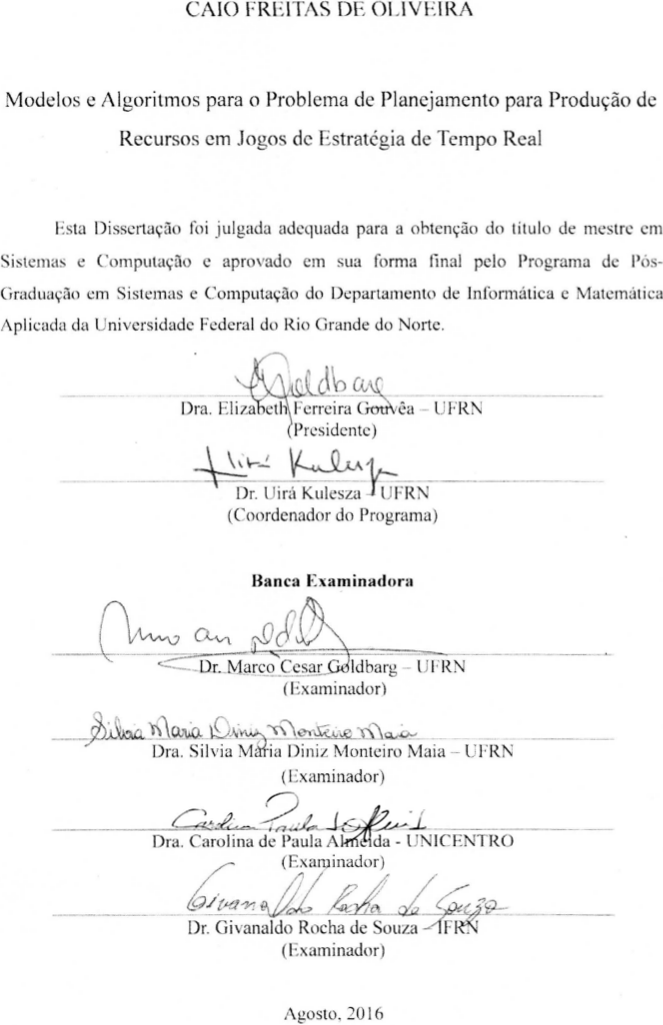
\includegraphics{Imagens/folha-aprova.png}
\end{figure}
%\begin{folhadeaprovacao}
%	\setlength{\ABNTsignthickness}{0.4pt}
%	\setlength{\ABNTsignwidth}{10cm}
	%
%	% Informa��es gerais acerca do trabalho 
%	% (nome do autor, t�tulo, institui��o � qual � submetido e natureza)
%	\noindent 
%	Disserta��o de Mestrado sob o t�tulo \textit{\Title} apresentada por 
%	\text{\Author} e aceita pelo Programa de P�s-Gradua��o em Sistemas e Computa��o do Departamento de Inform�tica e Matem�tica Aplicada da Universidade Federal do Rio Grande do Norte,
%	sendo aprovada por todos os membros da banca examinadora abaixo especificada:
		%
%	% Membros da banca examinadora e respectivas filia��es
%	\assinatura
%	{
%		\Advisor\\
%		{\small Orientadora} 															\\ 
%		{\footnotesize
%			Departamento de Inform�tica e Matem�tica Aplicada																	\\
%		  	Universidade Federal do Rio Grande do Norte
%		}
%	}
	%
%	\assinatura
%	{
%		Dr. Marco C�sar Goldbarg 						 \\ 
%		{\footnotesize
%			Departamento de Inform�tica e Matem�tica Aplicada 																	 \\
%		  	Universidade Federal do Rio Grande do Norte
%		}
%	}
		%
%	\assinatura
%	{
%		Dra. Silvia Maria Diniz Monteiro Maia 						 \\ 
%		{\footnotesize
%			Departamento de Inform�tica e Matem�tica Aplicada 																	 \\
%		  	Universidade Federal do Rio Grande do Norte
%		}
%	}
%
%	\assinatura
%	{
%		Dra. Carolina Paula de Almeida 						 \\ 
%		{\footnotesize
%			Departamento de Ci�ncia da Computa��o 																	 \\
%		  	Universidade Estadual do Centro-Oeste
%		}
%	}
%
%	\assinatura
%	{
%		Dr. Givanaldo Rocha de Souza 						 \\ 
%		{\footnotesize
%
%			Instituto Federal de Educa��o, Ci�ncia e Tecnologia do Rio Grande do Norte
%		}
%	}
		%
%	\vfill
	%
%	\begin{center}
%		Natal-RN, 05 de Agosto de 2016.
%	\end{center}
%\end{folhadeaprovacao}